\subsection{Lifting and placing objects: slippage detection}
%\subsection{Slippage}
In order to apply enough force to lift an object, we detect if it
slips.

%Although controlling slippage can be useful in several
%manipulation tasks, we focus on avoiding slippage when lifting.

Sensing slippage is not an straight-forward task since the
phenomena is not quite understood. If we observe humans, our skin
has innervations that respond to fast motions on the surface.
These innervations are the Meissner's corpuscles. They are
specialized on detecting vibrations. Those vibrations are, in
principle, related to the catch and release effect caused by an
object sliding on the surface of the skin. This has inspired other
researchers to build tactile sensors with the capability of
detecting vibrations using accelerometers\cite{howe89sensing}.

In our case we do not rely on this principle. Instead, we measure
the change of the force applied on the direction of the lifting.

We illustrate this principle on the following experiment. We use
the the cylindrical bottle ($mass=0.179 Kg$, $diameter=92 mm$,
$height=216 mm$) shown in figure~\ref{fig:slipseq}. The robot
approaches the bottle by the side, touches it and subsequently
rotates the thumb to grab the object. Since it is the first time
it works with the bottle, it closes its thumb and index finger
gently until contact with the object is detected. At this point,
it closes the fingers more to deflect the sensors. This is
necessary in order to obtain reliable readings from forces applied
in directions parallel to the base of the sensors. In
figure~\ref{fig:tactileref} we can observe the direction of the
forces on the tactile sensors. In this experiment, we use only the
tactile sensors on the distal phalanges of the fingers. The force
normal to the tactile sensor surface is in the X direction, and
the ones parallel are in the plane Y-Z.

When the fingers are closed on the object, the forces in X
increase. The forces in Z (on the direction of gravity) and the
forces in Y also change due to the deformation of the sensors.
This deformation depends, at this point, on the angle of incident
between the tactile sensor and the surface of the object and not
on the weight.

When the robot starts moving its hand upwards, that is indicated
by the increment of elbow angle figure~\ref{fig:slip}, the force
in Z increases in magnitude because the weight of the object pulls
the sensors down. Assuming that the motion is linearly upwards and
that the object does not rotate, the force should remain somewhat
stable. The exception is at the beginning of the lifting where the
dynamics of the motion are noticeable. The event just described is
illustrated on the right side of figure~\ref{fig:slip}.

On the left side of figure~\ref{fig:slip}, we see that the
behavior is different. The total force goes back to zero while the
fingers are still closed. This is because the object slipped from
the hand. A sequence of images of the slippage is shown in
figure~\ref{fig:slipseq}. It is important to notice in this figure
that the bottle moves downwards but also towards the front. That
is, the bottle rotates on the finger tips of the hand.

If we now return to figure~\ref{fig:slip}, we can see the dynamics
of the sensors/object interaction. After the point B, in the
figure, the total force becomes negative because the friction with
the object pulls the sensors down. This event is indicated by an
increment on the elbow angle. While the total force is negative,
there is a slight positive slope on the force that indicates some
slippage. But more importantly, the angle between forces Z and Y
in the thumb changes smoothly showing the rotational slippage.
Subsequently, the object stops pulling down the tactile sensors
when it touches the table. At point C in figure~\ref{fig:slip},
the fingers are opened.


In order to detect slippage, we observe the total tactile force
while the fingers are closed and the arm moves upwards. If we
detect a positive slope, we conclude that there is slippage. We
can observe this in figure~\ref{fig:slip}. From point B to C there
is a large positive slope. The slope is presented on the top plot
for reference. From points E to F, there is a slight slip that
stops and the grasp stabilizes.

The response time of this slip detector is not as fast as it would
be required to adjust the force instantly. Instead, a new attempt
to lift the object is done if slippage has been detected.

[The current limitation of these sensors is that computation is
done off-board. However, the hardware on the sensors have the
capability of doing this calculation faster.]


\begin{figure}[htbp]
\centerline{
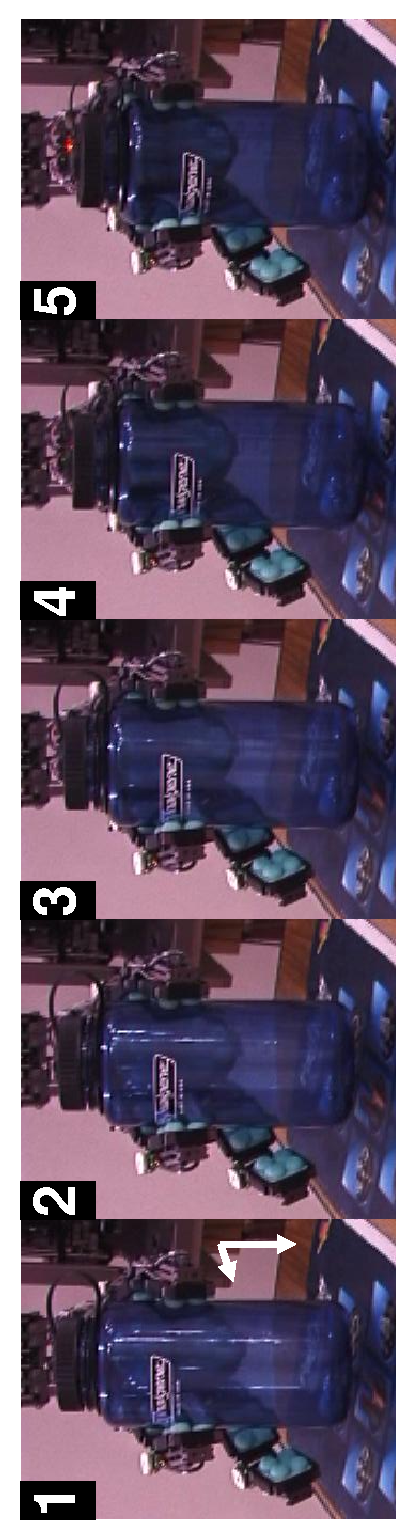
\includegraphics[height=\columnwidth, angle=270 ]{./figures/Slippage.eps}
} \caption[Bottle slipping]{From 1 to 5 we observe the bottle
slipping. The bottle moves downwards and towards the front. The
motion towards the front is not linear but circular.}
\label{fig:slipseq}
\end{figure}


It is important to remember that the data comes from a controlled
experiment where the lifting is done only with the thumb and the
index finger. Neither the palm nor the middle finger are used. In
general, this robot is designed to do whole body grasping as
opposed to precision grasping. In some cases, an object will come
in contact with the fingers on spots where the fingers are not
fully covered with the skin. In that case the slippage detection
is not possible.

\begin{figure*}[htbp]
\centerline{
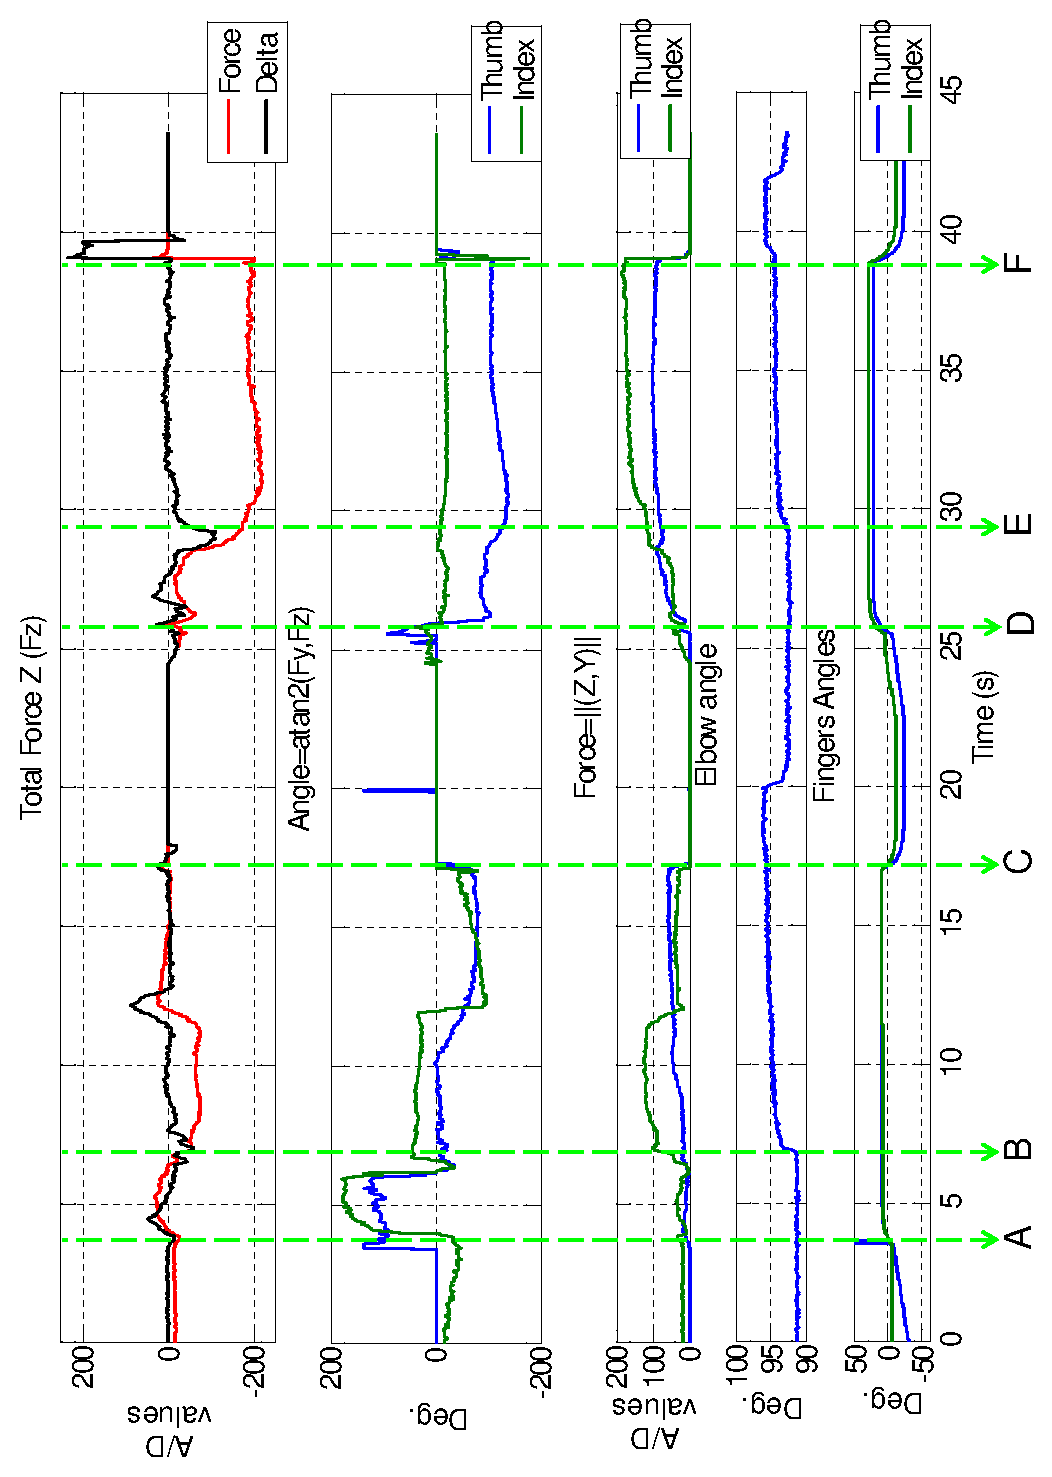
\includegraphics[height=\textwidth, angle=270 ]{./figures/ThesisSlipX.eps}
} \caption[Tactile forces when lifting an object]{Tactile forces
in two different lifting events. For details see
section~\ref{sec:slippage} } \label{fig:slip}
\end{figure*}



\subsection{Placing an object on a surface: applying forces to a held object}

Once the robot has an object in its hand, in order to interact
with the environment it is important to detect changes of forces
applied to the object. For instance, if the robot is holding an
object and wants to place it on a flat surface, like a table, it
is important to detect when they come in contact so an action can
be taken. Other examples where detecting external contact with a
held object include: using a hand tool, moving a cup towards our
mouth, etc.

OBRERO's tactile sensors are capable of measuring changes on the
forces applied to the object. In order to illustrate the principle
we present the following example. The robot grabs the bottle used
in section~\ref{sec:slippage}. Subsequently, it lifts the bottle
and then moves it back to the surface. The forces applied to the
object are monitored using the tactile sensors. When a large
change on the forces is detected in direction opposite to the
motion, the robot assumes that the object came in contact with a
surface and releases its grip. The robot is capable of detecting
this change at any time. For example, if we place our hand under
the bottle before the robot touches the surface, the robot will
able to detect this change on the tactile forces. This example is
presented in figure~\ref{fig:landing}.


It is arguable that this detection can also be done by force
sensors on the joints of the robot. However, this is generally
less sensitive because the effect of the change on forces needs to
be reflected on the joint. More importantly, a detailed model of
the forces acting on the joints needs to be implemented in order
to filter out the changes produced by other factors. Tactile
sensors are closer to the hand/object interaction making them more
sensitive and less complex at the moment of extracting the
information.

Figure~\ref{fig:twotaps} shows the response of the tactile sensors
to external forces on the object held. In this case, the robot is
holding an object and a person pushes the object from the bottom.
In order to see the response, we program the robot so that it does
not release the object. The plot on the top of
figure~\ref{fig:twotaps} shows the changes on the forces in the
direction of gravity.  We do not work with the absolute force but
with the differences because we are interested in the changes on
the force. The values showed have been filtered using a moving
average filter of size 8 and the sampling period is 100ms. The
bottom plot on figure~\ref{fig:twotaps} is the integration of the
data on the top plot, and it gives an idea of the time evolution
of the force applied. We can clearly observe that the force
increased because the object was pushed twice and the forces
applied had different intensity.

In order to detect the event of pushing or contacting the table
setting a threshold is enough, as it is illustrated on the top
plot of figure~\ref{fig:twotaps}.

\begin{figure}[htbp]
\centerline{
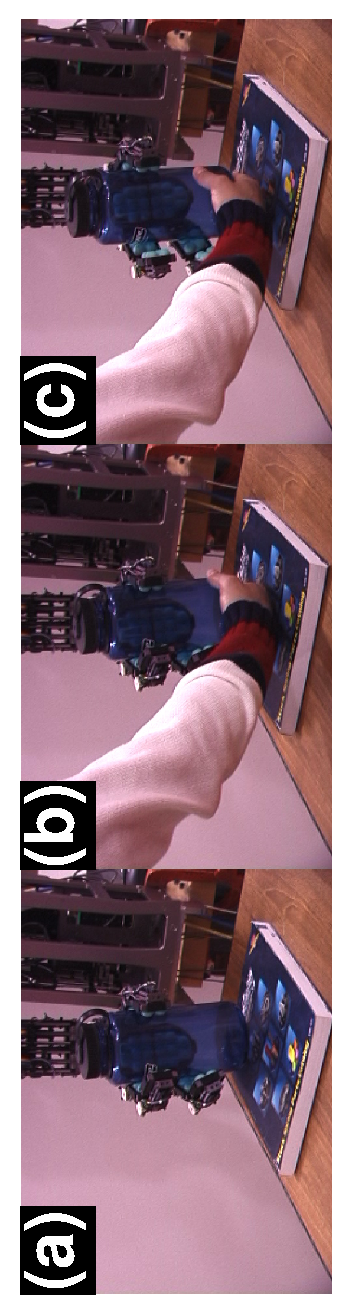
\includegraphics[height=\columnwidth, angle=270 ]{./figures/SeqHandDelivery.eps}
} \caption[Detection of forces applied to an object held by the
robot]{This sequence shows the robot detecting forces applied over
an object when holding it. This is useful to place objects over
surfaces. In (a) the robot is holding a bottle, in (b) a person is
touching the bottle from below and the robot detects this force.
As a consequence, the robot releases the object as shown in (c)}
\label{fig:landing}
\end{figure}

\begin{figure}[htbp]
\centerline{
\includegraphics[height=\columnwidth, angle=270 ]{./figures/2TapsX.eps}
} \caption[Pushing the bottle upwards twice]{Pushing the bottle
upwards twice. Top: Temporal difference of the total force in
direction on the gravity when the hand is holding an object. See
figure~\ref{fig:tactileref} for reference. Bottom: Integration of
the data on the top plot. It shows the changes on force when the
object was pushed.} \label{fig:twotaps}
\end{figure}

